\section{Introduction}
\label{sec:intro}

A numerical answer is trustworthy only when it can be traced to evidence in the current image. Visual measurement makes this requirement explicit: a model must identify the scale and boundary, reconstruct the local ticks, and connect each candidate to the state it denotes. Recent benchmarks show that vision--language models (VLMs) remain unreliable even when they recognize the instrument and unit~\cite{lin2026measurebench,jin2026scalebench}, but aggregate accuracy mixes perception, scale, localization, and grounding failures.

We focus on the correspondence between a numerical hypothesis and its image-specific state. For candidates 38.70 and 38.25\,$^{\circ}$C, a conventional interface requires the model to construct each position on the photographed scale. A \emph{physicalized} interface draws those states instead. Image, question, values, order, and scoring remain matched; only the denoted states become visible. In Fig.~\ref{fig:teaser}, the three-model majority rejects the correct symbolic candidate but selects it after physicalization.

\begin{figure}[t]
  \centering
  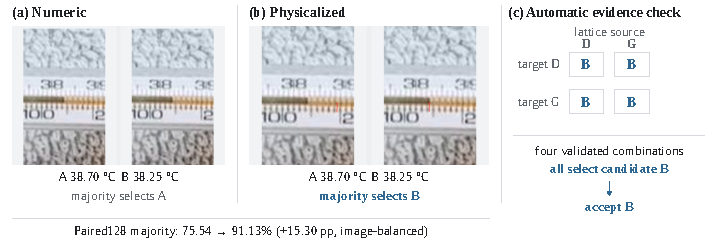
\includegraphics[width=\textwidth]{fig1_teaser.pdf}
  \Description{Three views of one thermometer example compare the same numerical candidates, candidate states drawn on the photographed scale, and an automatic check using four target-lattice combinations. The Numeric majority is incorrect and the Physicalized majority is correct.}
  \caption{\textbf{Same numbers, different access to their physical states.} Numeric presents two symbolic candidates; Physicalized renders the same values on the photographed scale. In this held-out example, the three-model majority changes from an incorrect to a correct choice. The automatic method tests the candidate across four validated target--lattice combinations. Source image adapted from MeasureBench~\cite{lin2026measurebench}, licensed under CC BY-SA 4.0; cropped and annotated by the authors.}
  \label{fig:teaser}
\end{figure}

This discontinuity isolates a \emph{symbol-to-state binding gap}. The map from value $v$ to visible state $g_I(v)$ changes with each image's branch, direction, phase, spacing, perspective, and operator. \dataset{} isolates it on \DatasetImages{} real images with human-refined local geometry. Across three matched interfaces, two candidate orders, and three VLMs, balanced gains are 8.40, 16.28, and 16.08 points for Doubao, Gemini, and Qwen. Three-model majority gains \MajorityBalancedGain{} points, removing 63.7\% of its remaining Numeric errors at call level. Calibration stays near Numeric, while the effect persists across reasoning budgets and major instrument families.

Oracle Physicalized uses human geometry; automatic verification must estimate both target and value--scale map. A proposal may remain self-consistent when target and lattice share a displacement. We therefore introduce \factorial{}: Doubao and Gemini propose target and lattice components, Qwen validates their evidence, and all four source combinations are resolved without another holistic answer. Precision mode requires executable components, four-way candidate agreement, and four-tick separation. The rule is selected on Dev69 and applied unchanged to held-out evaluation.

Our contributions are threefold:
\begin{itemize}
  \item We augment 200 real MeasureBench images with human-refined local geometry and matched Numeric, Calibrated, and Physicalized interfaces, forming \dataset{}. Its main matrix contains \FormalCalls{} controlled calls over \ImageDistancePairs{} image--distance pairs, complemented by an independent geometry audit spanning all \GeometryAuditFamilies{} families.
  \item We identify a cross-model binding gap: physicalizing identical numerical candidates raises majority accuracy by \MajorityBalancedGain{} points. The gap persists after scale calibration and increased reasoning, separates from target localization, and is larger on two-endpoint ruler spans.
  \item We propose \factorial{}, a training-free selective verifier that validates independently proposed components, recombines their sources, and accepts decisions stable across valid combinations and sufficiently separated in the physical state space. Its held-out precision is \FactorialTestPrecision\% across \FactorialTestImages{} images and \FactorialTestCoverage\% of ordered cells.
\end{itemize}
